\PassOptionsToPackage{unicode=true}{hyperref} % options for packages loaded elsewhere
\PassOptionsToPackage{hyphens}{url}
%
\documentclass[]{article}
\usepackage{lmodern}
\usepackage{amssymb,amsmath}
\usepackage{ifxetex,ifluatex}
\usepackage{graphicx}
\usepackage{wrapfig}
\usepackage{lscape}
\usepackage{rotating}
\usepackage{fixltx2e} % provides \textsubscript
\ifnum 0\ifxetex 1\fi\ifluatex 1\fi=0 % if pdftex
  \usepackage[T1]{fontenc}
  \usepackage[utf8x]{inputenc}
  \usepackage{textcomp} % provides euro and other symbols
\else % if luatex or xelatex
  \usepackage{unicode-math}
  \defaultfontfeatures{Ligatures=TeX,Scale=MatchLowercase}
\fi
% use upquote if available, for straight quotes in verbatim environments
\IfFileExists{upquote.sty}{\usepackage{upquote}}{}
% use microtype if available
\IfFileExists{microtype.sty}{%
\usepackage[]{microtype}
\UseMicrotypeSet[protrusion]{basicmath} % disable protrusion for tt fonts
}{}
\IfFileExists{parskip.sty}{%
\usepackage{parskip}
}{% else
\setlength{\parindent}{0pt}
\setlength{\parskip}{6pt plus 2pt minus 1pt}
}
\usepackage{hyperref}
\hypersetup{
            pdfborder={0 0 0},
            breaklinks=true}
\urlstyle{same}  % don't use monospace font for urls
\usepackage{graphicx,grffile}
\makeatletter
\def\maxwidth{\ifdim\Gin@nat@width>\linewidth\linewidth\else\Gin@nat@width\fi}
\def\maxheight{\ifdim\Gin@nat@height>\textheight\textheight\else\Gin@nat@height\fi}
\makeatother
% Scale images if necessary, so that they will not overflow the page
% margins by default, and it is still possible to overwrite the defaults
% using explicit options in \includegraphics[width, height, ...]{}
\setkeys{Gin}{width=\maxwidth,height=\maxheight,keepaspectratio}
\setlength{\emergencystretch}{3em}  % prevent overfull lines
\providecommand{\tightlist}{%
  \setlength{\itemsep}{0pt}\setlength{\parskip}{0pt}}
\setcounter{secnumdepth}{0}
% Redefines (sub)paragraphs to behave more like sections
\ifx\paragraph\undefined\else
\let\oldparagraph\paragraph
\renewcommand{\paragraph}[1]{\oldparagraph{#1}\mbox{}}
\fi
\ifx\subparagraph\undefined\else
\let\oldsubparagraph\subparagraph
\renewcommand{\subparagraph}[1]{\oldsubparagraph{#1}\mbox{}}
\fi

% set default figure placement to htbp
\makeatletter
\def\fps@figure{htbp}
\makeatother


\date{}

\begin{document}

\hypertarget{amsi}{%
\section{AMSI}\label{amsi}}

\hypertarget{introduction}{%
\subsection{Introduction}\label{introduction}}

Dans le cadre du cours d'Analyse et Modélisation de Systèmes
d'Information, il nous est demandé de réaliser l'analyse et la
modélisation du jeu \emph{Golden Quest} développé par la société Coding
Park. Ce jeu présente un personnage (Cody) sur une île au trésor. Le
joueur doit écrire une procédure informatique afin de déplacer Cody sur
l'île pour l'amener au trésor.

Le jeu est donc constitué de deux parties importantes : l'interface
visuelle (leçons, niveaux, plateaux de jeu) et l'interface de
programmation (procédures, instructions, expressions).

\hypertarget{moduxe9lisation-du-plateau-de-jeu}{%
\subsection{Modélisation du plateau de
jeu}\label{moduxe9lisation-du-plateau-de-jeu}}

La carte est constitué de cases qui sont caractérisées par leurs
coordonnées et leur nature (eau, gazon, pont). Les cases concrètes font
toutes parties d'un des trois groupes suivants: les cases accessibles
(sur lesquelles des entités peuvent évoluer), les obstacles
franchissable (par dessus lesquels Cody peut sauter) et les obstacles
infranchissable. La nature des cases est souvent forcée par la case
concrète, on peut difficilement envisager un buisson sur un pont ou de
l'eau.

Une Carte est associée à un Niveau qui est caractérisé par son nom ainsi
que des statistiques relativent au score du joueur. Chaque niveau peut
être suivi ou précédé par un autre niveau.

Un ensemble de Niveau constitue une Leçon, à leur tour caractérisées par
un nom et pouvant être suivies ou précédées d'autres leçons.

Au final l'ensemble des Leçon constitue un jeu associé au profil d'un
joueur dont la progression est défini par le dernier niveau qu'il a
atteint. Le joueur peut être soit un visiteur soir un membre inscrit
caractérisé par ses noms, age, email et mot de passe.

Les diagrammes de classes et d'objet ainsi que le niveau original se
trouvent en annexe.

\hypertarget{question-5.1}{%
\subsubsection{Question 5.1}\label{question-5.1}}

\begin{quote}
Établir une première version d'un diagramme de classes Uml qui fixe les
éléments principaux : le jeu est constitué d'une série de leçons
découpées en niveaux.
\end{quote}

\begin{figure}
\centering
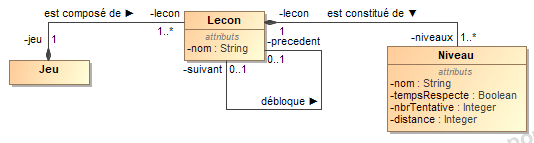
\includegraphics{./images_final/PlateauQ1.png}
\caption{Plateau jeu, leçons, niveaux}
\end{figure}

\hypertarget{question-5.2}{%
\subsubsection{Question 5.2}\label{question-5.2}}

\begin{quote}
Enrichir cette première version avec les détails nécessaires concernant
les joueurs et leurs profils, ainsi que les niveaux.
\end{quote}

\begin{figure}
\centering
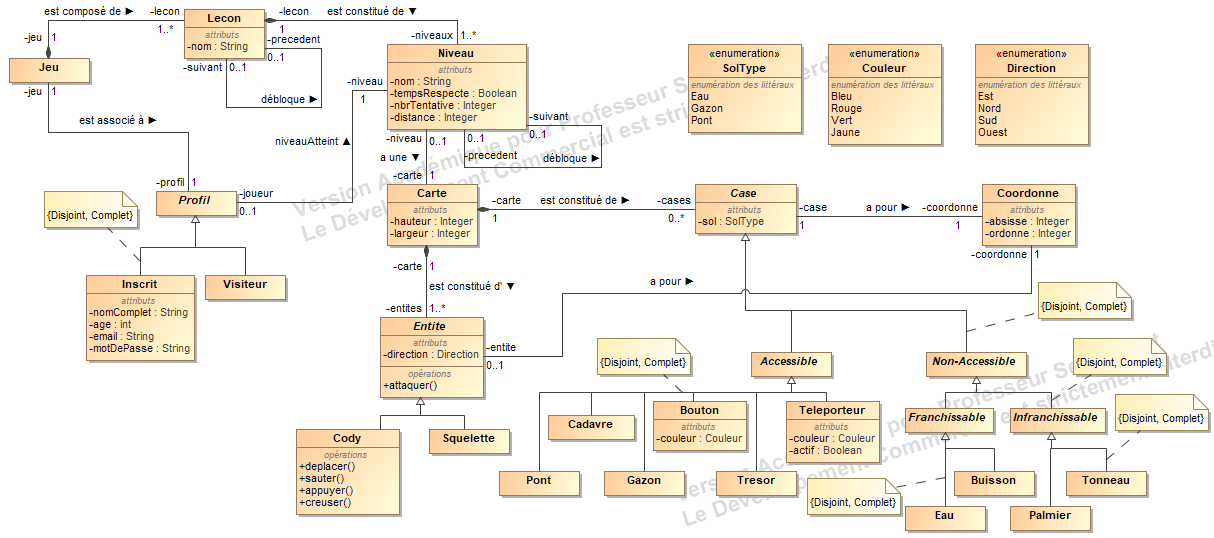
\includegraphics[angle=90, width=\textwidth, height=\textheight, keepaspectratio]{./images_final/PlateauQ2.png}
\caption{Plateau complet}
\end{figure}

\hypertarget{question-5.3}{%
\subsubsection{Question 5.3}\label{question-5.3}}

\begin{quote}
Spécifier les contraintes suivantes, soit à l'aide d'éléments
structurels dans le diagramme, éventuellement complétées par des
contraintes en OCL.
\end{quote}

\begin{enumerate}
\def\labelenumi{\arabic{enumi})}
\tightlist
\item
  Les coordonnées d'une case ne peuvent excéder les dimensions du
  niveau.
\end{enumerate}

\begin{verbatim}
context Carte
inv DansLesLimites:
self.cases->forAll(
    case.absice >= 0
    and case.coordonne.absice < self.largeur
    and case.coordonne.ordonne >= 0
    and case.coordonne.ordonne < self.hauteur
)
\end{verbatim}

\begin{enumerate}
\def\labelenumi{\arabic{enumi})}
\setcounter{enumi}{1}
\tightlist
\item Chaque niveau ne contient qu'un seul Cody, et qu'un seul coffre.
\end{enumerate}

\begin{verbatim}
context Carte
inv TresorUnique:
self.cases->select(
    case | case.oclIsTypeOf(Tresor)
).size() = 1
\end{verbatim}

\begin{verbatim}
context Carte
inv CodyUnique:
self.entites->select(
    entite | entite.oclIsTypeOf(Cody)
).size() = 1
\end{verbatim}

\begin{enumerate}
\def\labelenumi{\arabic{enumi})}
\setcounter{enumi}{2}
\tightlist
\item
  Un personnage ne peut pas se trouver sur un obstacle.
\end{enumerate}

\begin{verbatim}
context Entite
inv EntiteSurCaseAccessible: self.carte.cases.forAll->(
    case.coordonne = self.coordonne implies case.oclIsKindOf(Accessible)
)
\end{verbatim}

\begin{enumerate}
\def\labelenumi{\arabic{enumi})}
\setcounter{enumi}{3}
\tightlist
\item
  Deux personnages ne peuvent pas partager la même case.
\end{enumerate}

\begin{verbatim}
context Carte
inv CoordonneDesCasesUnique:
self.cases->forAll(
    c1, c2 | c1 <> c2 implies (c1.absice <> c2.absice or c1.ordonne <> c2.ordonne)
)
\end{verbatim}

Chaque case de la carte a des coordonnées unique et il ne peut y avoir
qu'au maximum une seule entité sur une case via l'unicité.

\begin{enumerate}
\def\labelenumi{\arabic{enumi})}
\setcounter{enumi}{4}
\tightlist
\item
  Le trésor doit se trouver sur du gazon.
\end{enumerate}

\begin{verbatim}
context Tresor
inv TypeGazon: self.sol = SolType.Gazon
\end{verbatim}

\begin{enumerate}
\def\labelenumi{\arabic{enumi})}
\setcounter{enumi}{5}
\tightlist
\item
  Un niveau doit toujours comporter deux tunnels de téléportation de
  même couleur, ou le tunnel unique doit être initialement fermé.
\end{enumerate}

\begin{verbatim}
context Teleporteur
inv TeleporteursParPairOuEteint:
self.carte.cases->select(
    tele | tele.oclIsTypeOf(Teleporteur)
           and tele.couleur = self.couleur
).size() = 2
or (
    not self.carte.cases->exists(
        tele | tele.oclIsTypeOf(Teleporteur)
               and tele <> self
               and tele.couleur = self.couleur
    )
    and not self.actif
)
\end{verbatim}

\begin{enumerate}
\def\labelenumi{\arabic{enumi})}
\setcounter{enumi}{6}
\tightlist
\item
  Un levier de téléportation ne peut être présent que s'il existe des
  tunnels de la même couleur.
\end{enumerate}

\begin{verbatim}
context Bouton
inv BoutonMemeCouleurQueTeleporteur:
self.carte.cases->exits(
	tele | tele.oclIsTypeOf(Teleporteur)
			and tele.couleur = self.couleur
)
\end{verbatim}

\begin{enumerate}
\def\labelenumi{\arabic{enumi})}
\setcounter{enumi}{7}
\tightlist
\item
  Les palmiers et les buissons doivent obligatoirement être posés sur du
  gazon (sinon, ils ne peuvent pas pousser).
\end{enumerate}

\begin{verbatim}
context Buisson
inv TypeGazon: self.sol = SolType.Gazon
\end{verbatim}

\begin{verbatim}
context Palmier
inv TypeGazon: self.sol = SolType.Gazon
\end{verbatim}

\hypertarget{question-5.4}{%
\subsubsection{Question 5.4}\label{question-5.4}}

\begin{enumerate}
\def\labelenumi{\arabic{enumi})}
\tightlist
\item Définir le niveau décrit à l'aide d'un Diagramme d'Objets Uml, en cohérence avec le Diagramme de Classe obtenu au terme de la Question 5.2.
\end{enumerate}

\begin{figure}
\centering
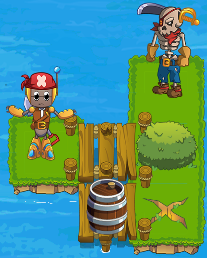
\includegraphics{./images_final/Niveau1.png}
\caption{Niveau à modéliser}
\end{figure}

\begin{figure}
\centering
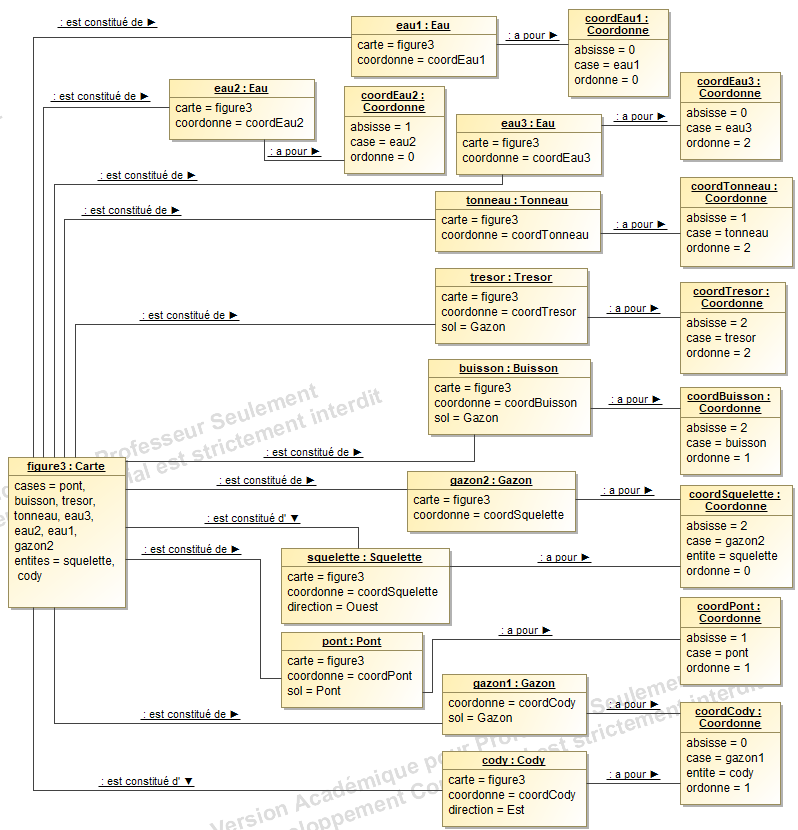
\includegraphics{./images_final/PlateauQ4.png}
\caption{Diagramme objet du niveau}
\end{figure}

\begin{enumerate}
\def\labelenumi{\arabic{enumi})}
\setcounter{enumi}{1}
\tightlist
\item
  Quelle propriété du jeu n'est pas satisfaite par ce niveau ?
\end{enumerate}

Le niveau n'est pas soluble. Cody n'a pas moyen de se déplacer à
l'emplacement du trésor.

\begin{enumerate}
\def\labelenumi{\arabic{enumi})}
\setcounter{enumi}{2}
\tightlist
\item
  Est-il possible de définir une contrainte OCL qui permette de vérifier cette propriété ? Pourquoi ?
\end{enumerate}

Non ce n'est pas possible de rédiger une contrainte OCL qui puisse
vérifier qu'un niveau est soluble. Les containtes OCL permettent de
définir des contraintes entre des objets compte tenu du diagramme de
classe auquels ils sont associés. Ce diagramme n'a aucune connaissance
de la logique fonctionnelle d'un niveau.

On peut tout au plus vérifier que le trésor se trouve à l'emplacement
actuel de cody ou à une distance d'une action de déplacement et que cody
ne se trouve pas entre deux squelettes ou plus. Au delà de ces cas de
base, une contrainte OCL n'est pas suffisante pour trouver un chemin
allat de Cody au trésor.

\hypertarget{moduxe9lisation-de-play}{%
\subsection{Modélisation de Play}\label{moduxe9lisation-de-play}}

Le langage utilisé dans le jeu est composé de procédures, elles-même
composées d'instructions qui font parfois appel à des expressions.

Il existe une procédure principal par programme, c'est celle qui est
exécutée en premier et qui arrêtera le jeu une fois finie.

Chaque instruction peut être soit simple soit composée. Les instructions
simple exécutent soit une procédure primitive existante dans GoldenQuest
soit une procédure définie par l'utilisateur. Parmi les actions
primitives, on différencie les actions de déplacement des autres. En
effet les actions de déplacement admettent un paramettre optionnel (tout
comme les procédure utilisateur si ce n'est que l'utilisateur peut
définir autant de paramettre qu'il le souhaite) alors que les autres
actions primitives n'ont pas de parametre. Les instructions composées
quant à elle regroupent une série d'autres instructions qui seront
jouées 0, 1 ou plusieurs fois en fonction de l'expression associé à
l'instruction composée. Parmi les instructions composés on retrouve les
conditions et les itérations.

Les expressions sont également simple ou composés. Les expressions
simple sont des litéraux ou des variable tandis que les expressions
composées permettent de regrouper ou d'effectuer des opérations sur
d'autres expressions.

Les différents diagrammes se trouvent en annexe.

\hypertarget{question-5.5}{%
\subsubsection{Question 5.5}\label{question-5.5}}

\begin{quote}
Établir une première version d'un diagramme de classe Uml qui fixe les
éléments principaux : un Program(me) Play est un ensemble de procédures
(dont l'une est la procédure principale).
\end{quote}

\begin{figure}
\centering
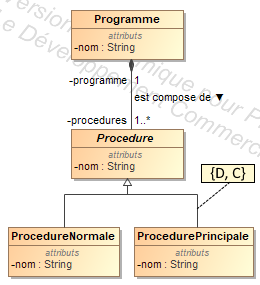
\includegraphics{./images_final/PlayQ5.png}
\caption{Play procédure}
\end{figure}

\hypertarget{question-5.6}{%
\subsubsection{Question 5.6}\label{question-5.6}}

\begin{quote}
Modéliser le concept de procédure à partir d'une classe Procedure.
\end{quote}

Non répondu

\hypertarget{question-5.7}{%
\subsubsection{Question 5.7}\label{question-5.7}}

Modéliser le concept d'expression comme indiqué en Section 3.3, à partir
d'une classe Expression.

\begin{figure}
\centering
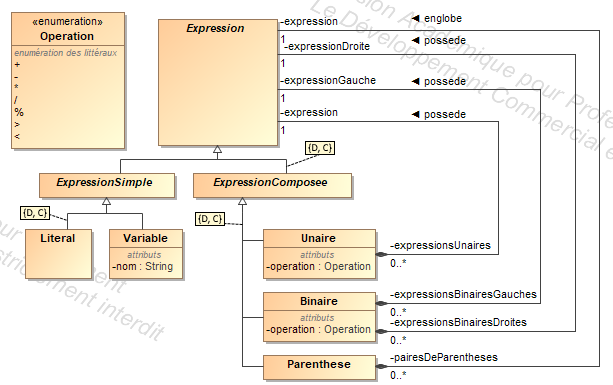
\includegraphics{./images_final/PlayQ7.png}
\caption{Play expression}
\end{figure}

\hypertarget{question-5.8}{%
\subsubsection{Question 5.8}\label{question-5.8}}

Modéliser le concept d'instruction comme indiqué en Section 3.2, à
partir d'une classe Instruction (qui fera usage de la classe
Expression).

\begin{figure}
\centering
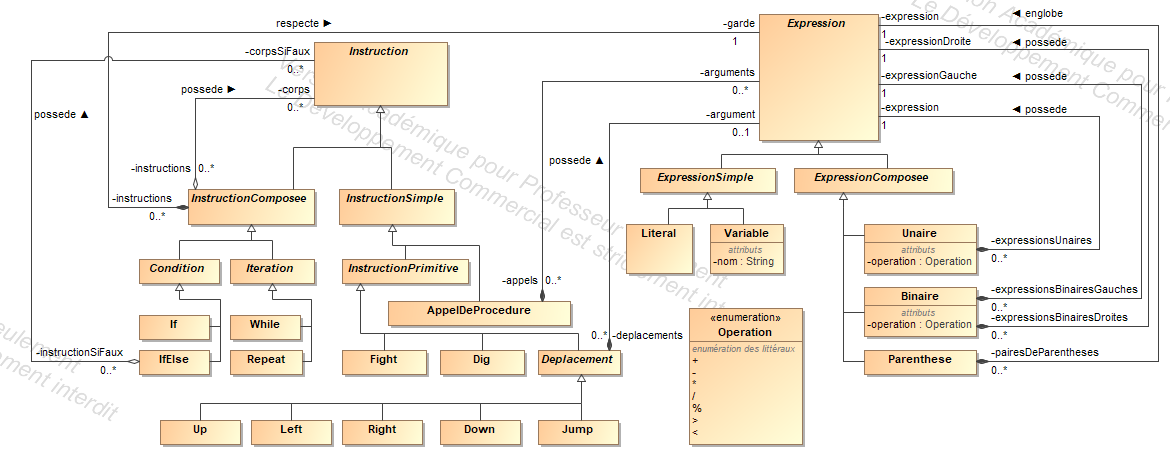
\includegraphics[angle=90, width=\textwidth, height=\textheight, keepaspectratio]{./images_final/PlayQ8.png}
\caption{Play instruction}
\end{figure}

\hypertarget{question-5.9}{%
\subsubsection{Question 5.9}\label{question-5.9}}

\begin{quote}
Spécifier les contraintes OCL suivantes
\end{quote}

\begin{enumerate}
\def\labelenumi{\arabic{enumi})}
\tightlist
\item
  Les noms des paramètres d'une procédure sont uniques.
\end{enumerate}

\begin{verbatim}
    context ProcedureNormale
    inv NomsParametresUniques:
    self.parametres.forAll -> (p1,p2 | p1 <> p2 implies p1.nom <> p2.nom)
\end{verbatim}

\begin{enumerate}
\def\labelenumi{\arabic{enumi})}
\setcounter{enumi}{1}
\tightlist
\item
  Les noms des procédures sont uniques au sein d'un Program(me).
\end{enumerate}

\begin{verbatim}
context Programme
inv NomProceduresUniques:
self.procedures.forAll->(p1,p2 | p1 <> p2 implies p1.nom <> p2.nom)
\end{verbatim}

\begin{enumerate}
\def\labelenumi{\arabic{enumi})}
\setcounter{enumi}{2}
\tightlist
\item
  Au moins une procédure doit être nommée Cody.
\end{enumerate}

\begin{verbatim}
context Programme
inv NomProcedureCody:
self.procedures.select->(p | p.nom = 'Cody').size() > 0
\end{verbatim}

\begin{enumerate}
\def\labelenumi{\arabic{enumi})}
\setcounter{enumi}{3}
\tightlist
\item
  S'il n'y a qu'une seule procédure dans le programme, l'instruction
  \texttt{dig()} doit apparaître au moins une fois.
\end{enumerate}

\begin{verbatim}
context Programme
pre: self.procedures.size() = 1
inv DigUneFois:
self.procedures.first()
    .instructions
    .any->(i | i.oclIsTypeOf(Dig))
\end{verbatim}

\hypertarget{question-5.10}{%
\subsubsection{Question 5.10}\label{question-5.10}}

\begin{quote}
Les expressions et les instructions obéissent à des contraintes afin de
garantir leur usage correct.
\end{quote}

\begin{itemize}
\item
  Identifier et préciser, en langage naturel, quelle(s) contraintes il
  faut imposer aux instructions pour qu'elles soient correctes.

  \begin{itemize}
  \tightlist
  \item
    Les expressions passées en argument dans un appel de procédure
    doivent être du même type que celles déclarées en parametre de la
    procédure.
  \end{itemize}
\item
  Même travail pour les expressions.

  \begin{itemize}
  \tightlist
  \item
    La contrainte explicitée au point précédent affecte également la
    classe Expression. Elles sont donc intimement liées.
  \end{itemize}
\item
  Indiquer quels éléments dans les questions de Play+ permettent de
  spécifier précisément ces contraintes.

  \begin{itemize}
  \tightlist
  \item
    Les éléments Type et Declaration qui sont liés aux Expressions vont
    permettre de spécifier cette contrainte OCL.
  \end{itemize}
\end{itemize}

\hypertarget{question-5.11}{%
\subsubsection{Question 5.11}\label{question-5.11}}

\begin{quote}
Donnez le code play et le diagramme UML de ce code qui permet de
terminer le niveau.
\end{quote}

\begin{figure}
\centering
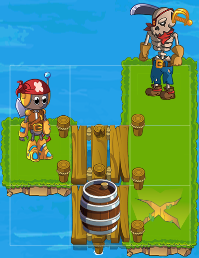
\includegraphics{./images_final/Niveau2.png}
\caption{Niveau à résoudre}
\end{figure}

\begin{verbatim}
procedure Cody() {
    right(2)
    fight()
    down()
    dig()
}
\end{verbatim}

\begin{quote}
Modélisez le code obtenu dans un diagramme objet.
\end{quote}

\begin{figure}
\centering
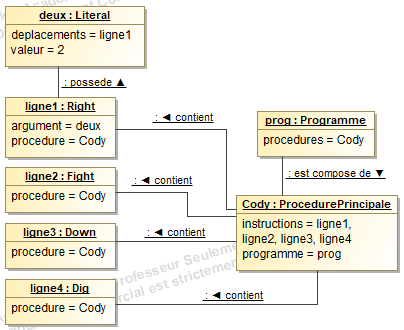
\includegraphics{./images_final/PlayQ11.png}
\caption{Diagramme objet}
\end{figure}

\hypertarget{moduxe9lisation-de-play-1}{%
\subsection{Modélisation de Play+}\label{moduxe9lisation-de-play-1}}

\hypertarget{question-5.12}{%
\subsubsection{Question 5.12}\label{question-5.12}}

\begin{quote}
Définir, à l'aide de l'Editeur de Niveau, un niveau original permettant
d'illustrer les concepts de boucles imbriquées, de portée de variables,
et de récursivitée.
\end{quote}

\begin{figure}
\centering
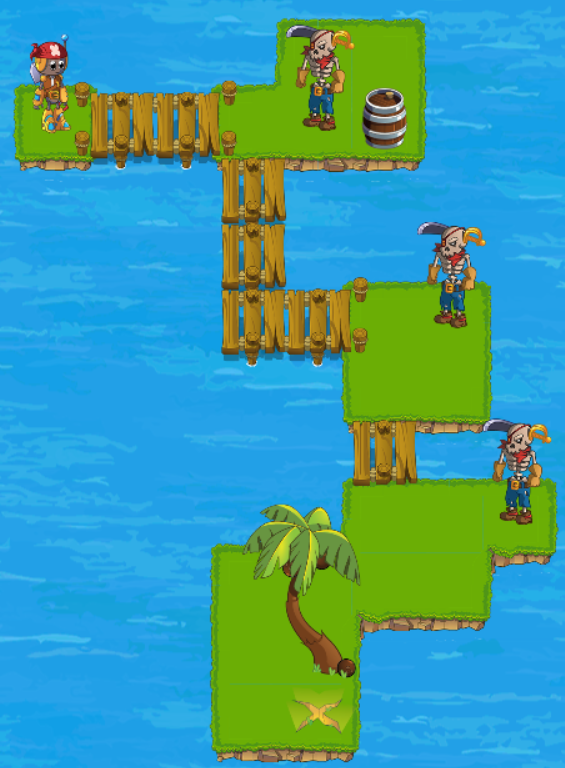
\includegraphics{./images_final/Play+Q12.png}
\caption{Play+ niveau original}
\end{figure}

\hypertarget{question-5.13}{%
\subsubsection{Question 5.13}\label{question-5.13}}

\begin{quote}
Modéliser le concept de Type, constitué des types primitifs, des
tableaux et des enregistrements. La modélisation doit pouvoir capturer
tous les exemples données en §4.1.
\end{quote}

\begin{figure}
\centering
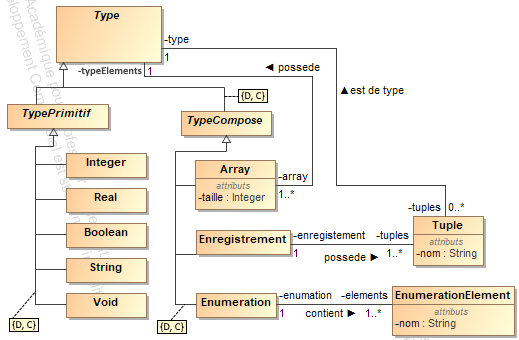
\includegraphics{./images_final/Play+Q13.png}
\caption{Play+ Type}
\end{figure}

\hypertarget{question-5.14}{%
\subsubsection{Question 5.14}\label{question-5.14}}

\begin{quote}
Modifier le détail d'un Program(me) afin qu'elle réponde à la nouvelle
définition : un Program(me) est constituée d'un ensemble de déclarations
(cf.~Section 4.2), et modéliser le concept de Declaration.
\end{quote}

\begin{figure}
\centering
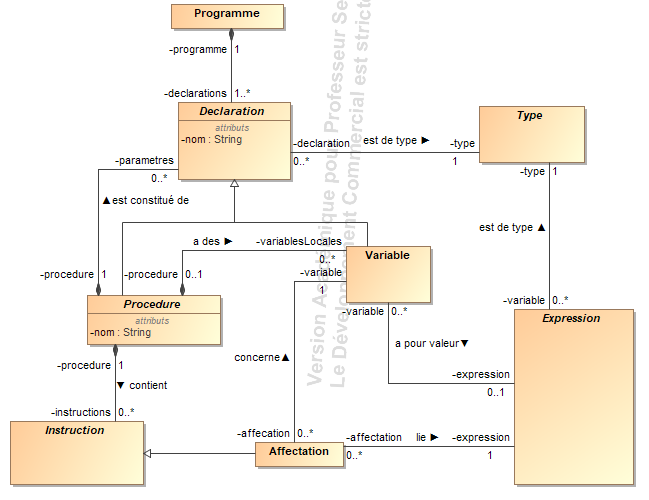
\includegraphics{./images_final/Play+Q14.png}
\caption{Play+ Déclaration}
\end{figure}

\hypertarget{question-5.15}{%
\subsubsection{Question 5.15}\label{question-5.15}}

\begin{quote}
Modifier le détail du concept Instruction afin d'ajouter les nouveaux
éléments définis en Section 4.3.
\end{quote}

\begin{figure}[ht]
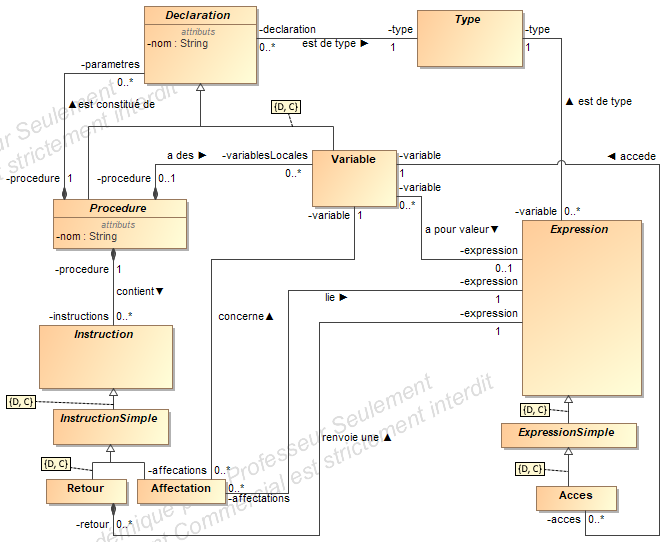
\includegraphics{./images_final/Play+Q15.png}
\caption{Play+ Instruction}
\end{figure}

\hypertarget{question-5.16}{%
\subsubsection{Question 5.16}\label{question-5.16}}

\begin{quote}
Modifier le détail du concept Expression afin de refleter les
modifications définis en Section 4.3.
\end{quote}

\begin{figure}
\centering
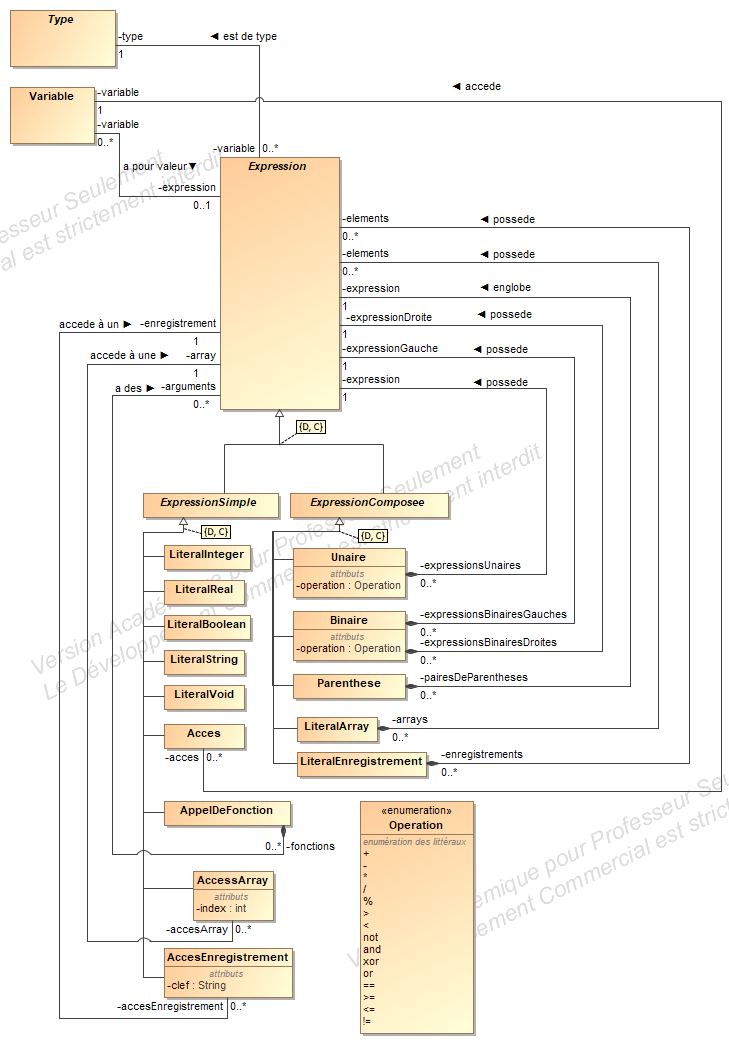
\includegraphics{./images_final/Play+Q16.png}
\caption{Play+ Expression}
\end{figure}

\hypertarget{question-5.17}{%
\subsubsection{Question 5.17}\label{question-5.17}}

\begin{quote}
Spécifier une contrainte Ocl permettant de vérifier qu'une déclaration
de type est bien formée :
\end{quote}

\begin{enumerate}
\def\labelenumi{\arabic{enumi})}
\tightlist
\item
  la liste de champs d'un enregistrement est non-vide ;
\end{enumerate}

\begin{verbatim}
context Enregistrement
inv listeChampsNonVide:
self.tuples->forAll(t | not OCLIsUndefined(t.nom))
\end{verbatim}

\begin{enumerate}
\def\labelenumi{\arabic{enumi})}
\setcounter{enumi}{1}
\tightlist
\item
  un tableau comporte au moins une dimension qui doit être strictement
  positive.
\end{enumerate}

\begin{verbatim}
context Array
inv tailePositive: self.taille >= 0
\end{verbatim}

\hypertarget{question-5.18}{%
\subsubsection{Question 5.18}\label{question-5.18}}

\begin{quote}
Spécifier une contrainte Ocl vérifiant l'unicité des déclarations au
sein de leur contexte :
\end{quote}

\begin{itemize}
\tightlist
\item
  Les noms de variables au sein d'une (instance d') Action;
\end{itemize}

Non répondu, quelle différence avec une variable locale ?

\begin{itemize}
\tightlist
\item
  les noms de variables déclarées au sein d'une procédure ;
\end{itemize}

\begin{verbatim}
context Procedure
inv variableLocalesUnique:
self.variablesLocales->forAll(
    v1, v2 | v1 <> v2 implies v1.nom <> v2.nom
)
\end{verbatim}

\begin{itemize}
\tightlist
\item
  les noms de variables déclarées au sein d'un corps de procédure ;
\end{itemize}

Non répondu, quelle différence avec une variable locale ?

\begin{itemize}
\tightlist
\item
  les noms des champs au sein d'un enregistrement.
\end{itemize}

\begin{verbatim}
context Enregistrement
inv nomChampUnique:
self.tuples->forAll(
    t1, t2 | t1 <> t2 implies t1.nom <> t2.nom
)
\end{verbatim}

\hypertarget{question-5.19}{%
\subsubsection{Question 5.19}\label{question-5.19}}

\begin{quote}
Spécifier en Ocl le contrat Ocl sur une opération type(exp : Expression)
: Type qui renvoie le type d'une expression :
\end{quote}

\begin{itemize}
\tightlist
\item
  Le type des littéraux est le type qui leur correspond (par exemple,
  true a pour type Booleen, 1 a pour type Entier, ``aa'' a pour type
  String) ;
\end{itemize}

\begin{verbatim}
context LiteralInteger
inv typeLiteralIntegerCorrect:
self.type.oclIsKindOf(Integer)

context LiteralString
inv typeLiteralStringCorrect:
self.type.oclIsKindOf(String)

context LiteralVoid
inv typeLiteralVoidCorrect:
self.type.oclIsKindOf(Void)

context LiteralReal
inv typeLiteralRealCorrect:
self.type.oclIsKindOf(Real)

context LiteralBoolean
inv typeLiteralBooleanCorrect:
self.type.oclIsKindOf(Boolean)

\end{verbatim}

\begin{itemize}
\tightlist
\item
  Le type d'une expression unaire est lié au type de son opérateur, à
  condition que sa sous-expression corresponde (par exemple, -1 doit
  avoir une sous-expression de type entier ou réel, et not b impose que
  b soit de type booléen) ;
\end{itemize}

\begin{verbatim}
\end{verbatim}

\begin{itemize}
\tightlist
\item
  Le type d'une expression binaire est lié au type de son opérateur
  (similaire au cas unaire, à vous de trouver des exemples pertinents) ;
\end{itemize}

\begin{verbatim}
context Binaire
pre: self.type.oclIsTypeOf(Boolean)
def operateursBooleensBinaire: Bag(Operation) = {Operation.and, Operation.not, Operation.xor, Operation.or}
inv expressionBinaireTypeBooleen: 
self.type = self.expressionGauche AND self.type = self.expressionDroite AND operateursBooleensBinaire.any->(o | o.operation = self.operation)

context Binaire
pre: self.type.oclIsTypeOf(Integer) OR self.type.oclIsTypeOf(Real)
def operateursNombresBinaire: Bag(Operation) = {Operation.+, Operation.-, Operation.*, Operation./, Operation.%, Operation.<, Operation.>, Operation.<=, Operation.>=, Operation.==, Operation.!=}
inv expressionBinaireTypeIntegerReal: 
(self.expressionGauche.type.oclIsTypeOf(Integer) OR self.expressionGauche.type.oclIsTypeOf(Real)) 
AND 
(self.expressionDroite.type.oclIsTypeOf(Integer) OR self.expressionDroite.type.oclIsTypeOf(Real))
AND 
operateursBooleensBinaire->any(o | o.operation = self.operation)
\end{verbatim}

\begin{itemize}
\tightlist
\item
  Le type d'une expression parenthésée est le type de sa sous-expression
  ;
\end{itemize}

\begin{verbatim}
context Parenthese
inv contrainteExpressionParenthesee:
self.type = expression.type
\end{verbatim}

\begin{itemize}
\tightlist
\item
  Le type d'un accès à une variable est son type de déclaration ;
\end{itemize}

\begin{verbatim}
context Acces
inv contrainteAcces:
self.type = self.variable.type
\end{verbatim}

\begin{itemize}
\tightlist
\item
  Le type d'une expression gauche correspondant à l'accès à un champ est
  le type de sa déclaration dans l'enregistrement ;
\end{itemize}

Non représenté sur le schéma global.

Un enregistrement serait représenté par une expression litérale
(LiterayRecord) ayant le type Enregistrement et serait une spécification
d'une expression composite. Cette expression composite serait composée
d'autres expression (ses pairs clé, valeur) pour lequels la clé serait
de type String et la valeur du type de la valeur associé au tuple dont
le nom est la clé pour l'enregistrement associé.

L'accès à une valeur d'un enregistrement serait une expression simple
ayant pour type le type de la valeur du champ de l'enregistrement
associé (association par un enregistrement litéral ou par une variable
de type Enregistrement). Cet accès serait composée d'une clé, une
expression simple de type String, devant exister dans l'enregistrement.

\begin{itemize}
\tightlist
\item
  Le type d'une expression gauche d'accès à une case de tableau est le
  type de déclaration du tableau.
\end{itemize}

Non représenté sur le schéma global.

Un tableau serait représenté par une expression litérale (LiteralArray)
ayant le type Array et qui serait une spécification d'une expression
composite. Cette expression composite serait composée d'autres
expressions (ses éléments) tous du même type que le type associé au type
Array du LiteralArray.

L'accès à un élément d'un tableau serait une expression simple ayant
pour type le type des éléments de l'Array associée (association par un
tableau llitéral ou par une variable de type Array). Cet accès serait
composé d'un indice, une expression simple de type Integer, devant se
trouver dans les limites du tableau.

\hypertarget{question-5.20}{%
\subsubsection{Question 5.20}\label{question-5.20}}

\begin{quote}
Spécifier le contrat Ocl sur une opération estValide() : boolean qui
vérifie qu'une instruction est valide :
\end{quote}

\begin{itemize}
\tightlist
\item
  Les gardes des instructions composées doivent posséder un type booleen
  ;
\end{itemize}

\begin{verbatim}
context InstructionComposee
inv GardeBooleenne:
self.garde.type.oclIsTypeOf(Boolean)
\end{verbatim}

\begin{itemize}
\tightlist
\item
  Les paramètres des instructions d'actions doivent être entier ;
\end{itemize}

\begin{verbatim}
context Deplacement
inv ArgumentEntier:
self.argument.type.oclIsTypeOf(Integer)
\end{verbatim}

\begin{itemize}
\tightlist
\item
  Les parties gauche et droite d'une affectation doivent être de même
  type ;
\end{itemize}

\begin{verbatim}
context Affectation
inv VariableEtValeurOntLeMemeType:
self.expression.type = self.variable.type
\end{verbatim}

\begin{itemize}
\tightlist
\item
  Le type de retour d'une procédure doit toujours être void.
\end{itemize}

\begin{verbatim}
context AppelDeProcedure
inv ProcedureTypeVoid
self.procedureAppelee.type.OclIsTypeOf(Void)
\end{verbatim}

\hypertarget{question-5.21}{%
\subsubsection{Question 5.21}\label{question-5.21}}

\begin{quote}
Les instructions d'actions primitives de déplacement obéissent à une
logique particulière en présence de certains éléments. En supposant
l'existence d'une opération prec mouv() : Déplacement qui retourne la
direction du dernier déplacement effectué, spécifier les contrats Ocl
sur l'ensemble de ces instructions :
\end{quote}

\begin{itemize}
\tightlist
\item
  Lorsqu'une telle instruction tente d'accéder une case où se trouve un
  obstacle, le déplacement n'est pas effectué ;
\end{itemize}

\begin{verbatim}
context Cody::prec_move(dir: Direction)
inv SeDeplaceSurUneCaseNonAccessible:
pre: not self.carte.cases->any(case |
    case.coordonne.abscisse = self.coordonne.abscisse + (
        dir = Direction.Est implies 1
        or dir = Direction.Ouest implies -1
        or (dir <> Direction.Est and dir <> Direction.Ouest) implies 0)
    and case.coordonne.ordonne = self.coordonne.ordonne + (
        dir = Direction.Sud implies 1
        or dir = Direction.Nord implies -1
        or (dir <> Direction.Sud and dir <> Direction.Nord) implies 0)
    and case.OclIsKindOf(Accessible))
post: self.coordonne = self.coordonne@pre
\end{verbatim}

\begin{itemize}
\tightlist
\item
  Lorsqu'une telle instruction tente d'accéder une case où se trouve un
  tunnel, on ressort dans la case suivant le dernier mouvement à partir
  de l'autre tunnel ;
\end{itemize}

Non répondu

\begin{itemize}
\tightlist
\item
  Lorsqu'on saute dans une direction à partir d'une case, on se atterit
  deux cases plus loin dans la même direction ; s'il y a un obstacle
  dans la case suivante, on reste sur place.
\end{itemize}

Non répondu

\hypertarget{question-5.22}{%
\subsubsection{Question 5.22}\label{question-5.22}}

\begin{quote}
Donner le code Play+ permettant de résoudre votre niveau original défini
dans la Question 5.12.
\end{quote}

\end{document}
